\chapter{Analýza}

\section{Prostředí}

Požadavky na použité prostředí jsou určeny převážně požadavky frameworku OpenSMT, pod nějž tato práce spadá. OpenSMT --- a~tudíž i~tento projekt --- je programován v~jazyce C++, konkrétně ve verzi C++11. Práce byla vyvíjena a~testována na operačním systému s~linuxovým jádrem nad architekturou x64. Jelikož si nejsme vědomi toho, že bychom použili vlastnosti jazyka specifické pro tuto konfiguraci, věříme, že náš kód bude možné bez větších potíží zprovoznit i~na jiných platformách a~operačních systémech.

\section{Fungování SMT řešičů}\label{smt}

Vzhledem k~podobnostem mezi SAT a~SMT není překvapením, že SMT řešiče využívají schopností SAT řešičů. Přechod mezi rozhraním termů teorie a~SAT řešičem zpravidla probíhá jedním ze dvou základních způsobů \cite{Nieuwenhuis05}.

První přístup se nazývá \emph{hladový}. Hladové SMT řešiče operují ve dvou krocích. V~prvním převedou celou vstupní formuli na ekvisplnitelnou booleovskou formuli. Druhý krok pak již spočívá jen v~předání této formule existujícímu SAT řešiči. Pokud bychom tedy pracovali například s~aritmetikou nad osmibitovými čísly, mohli bychom reprezentovat každou proměnnou osmi binárními proměnnými a~aritmetické operace převézt na odpovídající sekvence logických operací.

Nespornou výhodou hladových řešičů je možnost použití již existujících metod implementovaných na řešení SAT. Pro některé teorie se také hladové řešiče ukazují být rychlejší než jejich alternativy. Jejich největší problém pak obecně spočívá v~překladu literálů teorie do booleovských formulí. Ten musí být zkonstruován samostatně pro každou teorii, a~navíc může v~závislosti na teorii produkovat formule výrazně (často exponenciálně) delší, než byl původní vstup. Efektivní převody existují např. pro EUF s~omezenou doménou \cite{randal02}, obecně však hladový přístup není příliš rozšířený.

Jeho protějškem je takzvaný \emph{líný přístup}. Líný přístup se nesnaží měnit strukturu vstupní formule; namísto toho je každý predikát abstrahován pomocí nové binární proměnné. Když pak SAT řešič rozhodne o~ohodnocení těchto proměnných, oznámí toto rozhodnutí dedikovanému \emph{řešiči teorie}\footnote{Použitím pojmu \emph{řešič} bez přívlastku rozumíme v~této práci právě řešič teorie.}. Řešič teorie je schopen určit, zda je dané ohodnocení konzistentní, tzn.~dokáže rozhodnout o~splnitelnosti nějaké konjunkce literálů této teorie. SAT řešič potom hledá platná ohodnocení, dokud nenajde takové, které řešič teorie prohlásí za konzistentní.

Ve prospěch líných SMT řešičů svědčí fakt, že pro danou teorii často existují dobře známé postupy na ověření konjunkce literálů. Pro LA například můžeme využít metod lineárního programování, řešič teorie DL řeší STP (viz.~\ref{stp}) a~podobně. Líné řešiče však mohou ztrácet efektivitu zejména v~důsledku \emph{slepého prohledávání} \cite{Moura04}, kde hlavní řešič rozhoduje o~hodnotě predikátů, aniž by a~priori věděl o~důsledcích těchto ohodnocení v~rámci teorie, což může vést k~nutnosti vyzkoušet velké množství ohodnocení, než je nalezeno nějaké, které je s~teorií konzistentní.

V~roce 2004 navrhli Gazinger a~kol. nový přístup zvaný \emph{DPLL(T)} \cite{Gazinger04}. DPLL($T$) má koncepčně blíže k~línému vyhodnocování, integruje však těsněji hlavní řešič s~řešiči teorie. Místo toho, aby využíval řešiče teorie až po nalezení nějakého ohodnocení, průběžně mu oznamuje dosavadní rozhodnutí a~periodicky se ho ptá na splnitelnost právě dosazené konjunkce. Řešič teorie pak kromě kontroly splnitelnosti také oznamuje hlavnímu řešiči důsledky této konjunkce. Tím jsme schopni dříve opustit větve rozhodovacího stromu nekonzistentní s~teorií. 

V~jádru tohoto přístupu stojí obecný DPLL($X$) engine\footnote{Autoři práce si nejsou vědomi vhodného českého překladu, používají proto všeobecně známý anglický termín v~jeho nezměněné podobě.} , využívající DPLL \cite{Davis60} postupu pro SAT řešiče. Tento engine rozhoduje o~ohodnocení termů a~stará se o~zpracování booleovské logiky během výpočtu. K~tomu nemusí mít žádné znalosti o~konkrétní teorii. Přijímá totiž jako parametr specializovaný řešič teorie \Solver, který už je schopen s~teorií pracovat. Dosazením \Solver dané teorie $T$ za parametr $X$ pak vytvoříme konkrétní instanci DPLL($T$). Hlavní engine přitom v~průběhu výpočtu komunikuje se \Solver.

Stejně jako u~líných řešičů, v~DPLL($T$) abstrahuje \Solver literály teorie za běžné booleovské proměnné, se kterými může DPLL($X$) pracovat. Než tedy začne samotný výpočet, musí být \Solver poskytnuta vstupní formule, aby bylo možné provést tuto transformaci. Jakmile pak engine během výpočtu rozhodne o~pravdivostní hodnotě některého abstrahovaného literálu, okamžitě toto rozhodnutí oznámí řešiči teorie. Ten musí rozhodnout, zda je ohodnocení konzistentní s~předešlými ohodnocenými literály. Může navíc objevit nějaké důsledky tohoto ohodnocení v~teorii. Výsledek \Solver předá zpět DPLL($X$), který podle něj určí další postup. 

Pokud se ukáže ohodnocení jako konzistentní, pokračuje v~rozhodování o~pravdivosti dalších literálů. Bere přitom ohled na nalezené důsledky. Je-li naopak ohodnocení sporné, musí analyzovat příčinu sporu a~vrátit se zpět do stavu, kdy byl ještě konzistentní. \Solver musí být pro tento případ schopen předávat informace vysvětlující jeho rozhodnutí, poněvadž jako jediný zná vztahy mezi abstrahovanými proměnnými. Samozřejmě se pak od něj vyžaduje také schopnost vrátit se do předchozího stavu, tj.~zapomenout určitý počet nejpozději přidaných ohodnocení.

Vzhledem k~těmto požadavků na \Solver dospěli autoři frameworku~\cite{Gazinger04} k~následujícímu rozhraní propojujícím řešič teorie s~DPLL($X$):

\begin{description}
	\item[Initialize(L: množina literálů).] Inicializuje \Solver množinou literálů $L$, které se vyskytují v~problému.
	\item[SetTrue(l: L-literál): množina L-literálů.] Pokud se $l$ ukáže konzistentní s~předchozími ohodnoceními, přidá ho do seznamu zadaných literálů a~vrátí nějakou množinu důsledků tohoto přidání. V~opačném případě vyvolá výjimku vyjadřující spornost $l$ s~dosud zadanými literály. S~ohledem na výkonnost řešiče může být vrácená množina důsledků neúplná (popř. úplně prázdná).
	\item[IsTrue?(l: L-literál): boolean.] Vrátí \emph{true} právě tehdy, když $l$ je důsledkem seznamu přidaných literálů. Vrací \emph{false}, pokud je důsledkem tohoto seznamu $\neg l$, nebo pokud z~něj nevyplývá ani $l$, ani $\neg l$.
	\item[Backtrack(n: přir. číslo).] Odstraní posledních $n$ hodnot ze seznamu zadaných literálů. $n$ nesmí být větší než velikost tohoto seznamu.
	\item[Explain(l: L-literál): množina L-literálů.] Vrátí pokud možno co nejmenší podmnožinu zadaných literálů, z~jejichž konjunkce plyne $l$. Pro $l$ musí platit, že je důsledkem nějaké takové podmnožiny, tedy musí být obsažen v~návratové hodnotě nějakého volání \icode{SetTrue($l'$)} takového, že $l'$ nebylo zahozeno žádným následným voláním \icode{Backtrack}.
\end{description}

Při použití tohoto rozhraní \Solver nemusí nic vědět o~implementaci DPLL($X$) enginu. Framework je tedy velice modulární a~snadno rozšiřitelný o~nové teorie. Vyžadujeme pouze, aby byl \Solver schopný inkrementálně přijímat a~odebírat jednotlivé literály teorie. Tento postup se v~praxi ukazuje jako efektivnější než dostupné alternativy. Většina dnes rozšířených SMT řešičů --- včetně námi používaného OpenSMT2 --- je tedy založena na metodě DPLL($T$).

\section{Převod STP na grafový problém}\label{graf}

Velkou rozšířenost STP můžeme mimo jiné přisoudit tomu, že jsme schopni ho efektivně řešit. Jelikož se problém skládá výlučně z~lineárních omezení, mohli bychom na první pohled využít metod lineárního programování, jako je například simplexový algoritmus. Tyto metody jsou schopny řešit i~mnohem komplexnější problémy, avšak s~jejich výpočetní silou se pojí znatelně vyšší časová náročnost. Algoritmy specializované na STP se proto už od svého počátku \cite[Kapitola 2]{Dechter91} obracejí jiným směrem, a~to k~formalizmu teorie grafů. Přestože v~průběhu let vznikly různé metody řešení tohoto problému, všechny fungují na základě převedení množiny omezení na takzvaný \emph{omezující graf}.

\begin{definice}[Omezující graf]
	Nechť $\Pi$ je množina rozdílových omezení (\ref{eq:diff}). Omezujícím grafem této množiny rozumíme hranově ohodnocený orientovaný graf G takový, že vrcholy G tvoří proměnné vyskytující se v~$\Pi$ a~každému omezení $(x-y \leq c) \in \Pi$ odpovídá v~G hrana $\langle x,y\rangle$ s~ohodnocením $c$.
\end{definice}
\begin{pozn}
	Hranu $\langle x,y\rangle$ s~ohodnocením $c$ budeme značit $x \xrightarrow{c} y$. Orientovanou cestu z~$x$ do $y$ se součtem ohodnocení $k$ pak budeme značit $x \xrightarrow{k*} y$.
\end{pozn}

Pro úplnost dodejme, že dvojice proměnných se může vyskytovat v~libovolně mnoha omezeních. Omezující graf je tedy formálně orientovaným multigrafem. Vzhledem k~vzájemné bijekci mezi hranami grafu a~nerovnicemi problému budeme v~průběhu práce volně přecházet mezi oběma reprezentacemi. Příklad převedení množiny rozdílových omezení na odpovídající omezující graf ukazuje obrázek \ref{fig:graph}.

\begin{figure}
	\centering
	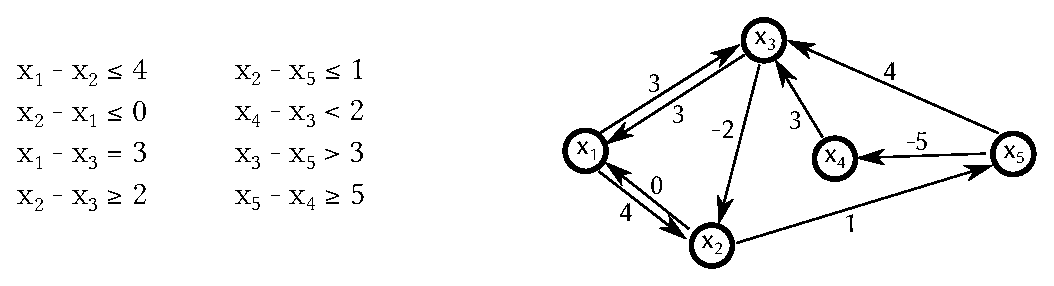
\includegraphics[width=\textwidth]{graph_example}
	\caption{Převod STP problému nad $\Z$ na omezující graf}
	\label{fig:graph}
\end{figure}

Převod do formy grafu je pro řešení problému zásadní. Umožňuje nám totiž formulovat následující klíčové tvrzení.

\begin{tvrz}[Dechter a~kol. \cite{Dechter91}]
	Nechť $\Pi$ je množina rozdílových omezení. Instance STP tvořená touto množinou je splnitelná právě tehdy, když omezující graf $\Pi$ neobsahuje záporné cykly.
\end{tvrz}
\begin{proof}
	Najdeme-li v~omezujícím grafu záporný cyklus obsahující vrchol $x$, sečtením všech nerovnic vyskytujících se v~tomto cyklu dostaneme $x-x \leq c < 0$, z~čehož je jasně problém nesplnitelný. Je-li na druhou stranu problém nesplnitelný, obsahuje $\Pi$ nějakou nerovnici $x - y \leq c$ takovou, že z~$\Pi$ vyplývá $y - x < -c$. Tato implikace znamená, že v~omezujícím grafu existuje cesta $y \xrightarrow{k*} x$ taková, že $k < -c$. Hrana $x \xrightarrow{c} y$ pak společně s~touto cestou tvoří záporný cyklus.
\end{proof}

Hledání splnitelnosti STP jsme tedy schopni převést na hledání záporného cyklu v~grafu (příklad převodu ukazuje obrázek \ref{fig:unsat}). To je problém, který dokážeme efektivně řešit. Využít můžeme např. některý algoritmus na hledání nejkratší cesty, kupříkladu Floydův-Warshallův algoritmus operující v~čase $\Theta(\abs{V}^3)$ nebo Bellmanův-Fordův algoritmus, který má časovou složitost $\Theta(\abs{V}\cdot\abs{E})$.

\begin{figure}
	\centering
	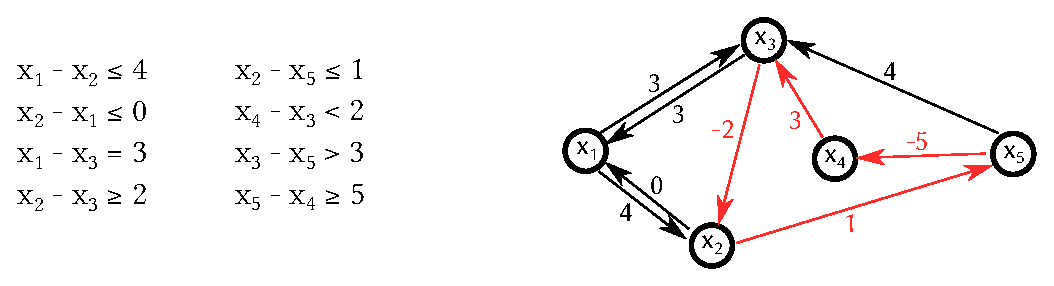
\includegraphics[width=\textwidth]{graph_unsat}
	\caption{Rozhodnutí o~nesplnitelnosti STP nalezením záporného cyklu}
	\label{fig:unsat}
\end{figure}

Tyto algoritmy však trpí pro náš účel zásadním nedostatkem. Jejich použití znamená, že po každém přidání nové hrany do grafu musí znovu proběhnout celé prohledávání. Tento postup není vhodný pro použití v~SMT řešičích, ve kterých je kladen velký důraz na inkrementalitu. V~následující sekci tedy podrobně rozebereme několik postupů pro řešení problémů SMT s~ohledem na DL a~motivujeme výběr námi použitého algoritmu. 

\section{Volba algoritmu}\label{alg}

Jak jsme ukázali v~předchozí sekci, ne všechny algoritmy na rozhodnutí STP jsou dobrou volbou pro použití v~kontextu SMT řešičů. Řešič teorie pro DPLL($T$) by měl efektivně podporovat dvě zásadní operace --- inkrementální přidávání literálů a~backtracking.

Na rozdíl od základního hladového přístupu, jak byl popsán v~sekci \ref{smt}, v~DPLL($T$) dostává \Solver informaci o~rozhodnutých ohodnoceních průběžně. Aby byly dříve odhaleny slepé větve v~rozhodovacím stromu, \Solver je průběžně dotazován na splnitelnost dosud provedených rozhodnutí. Pro zrychlení tohoto procesu je tedy vhodné, aby byl schopen pro výpočet využít výsledků z~předchozích dokončených výpočtů. Algoritmy, které nedokáží takto zakomponovat mezivýpočet podproblému, budou ze své podstaty méně výkonné na postupné sekvenci splnitelných ohodnocení.

Po nalezení nesplnitelného ohodnocení pak neopakuje engine celý výpočet, ale vrací se pouze do nejbližšího stavu, ve kterém bylo ohodnocení ještě splnitelné. Od řešiče teorie očekáváme, že je schopen efektivně zapomínat přidané literály, vracet se do předchozích stavů a~pokračovat z~nich ve výpočtu. %% FIXME: Better wording?
S~ohledem na tyto požadavky vzniklo několik algoritmů pro řešení SMT s~ohledem na DL. V~této práci se budeme zabývat převážně postupem založeným na vyčerpávající propagaci teorie, který postulovali v~roce 2005 Nieuwenhuis a~Oliveras \cite{Nieuwenhuis05}. Ten podrobně popisujeme v~sekci \ref{dpllt}. Existují ale i~další přístupy, kterými lze v~rámci DPLL($T$) problém řešit.

Jako možnou alternativu uveďme algoritmus, který prezentovali Wang a~kol. \cite{Wang05} a~jejichž řešič se koncepčně od našeho přístupu značně liší. Vychází z~Bellmanova-Fordova algoritmu, využitelného mimo jiné k~detekci záporných cyklů. Pomocí několika klíčových pozorování pak odstraňuje jeho nedostatky pro použití v~SMT řešičích. Zásadní změna spočívá v~inkrementalitě řešení. Běžný Bellmanův-Fordův algoritmus by musel pokaždé relaxovat všechny hrany grafu nezávisle na předchozích výpočtech. Jak ale ukázali autoři \cite{Wang05}, pokud nepotřebujeme hledat nutně nejkratší cesty, nemusí vrcholy grafu nutně začínat s~nekonečným potenciálem. Jejich řešič si tedy může ukládat délky nalezené v~jednom průběhu relaxačního algoritmu a~použít je jako výchozí hodnoty pro následující průběh. Tím se v~praxi podstatně sníží počet relaxací nutných ke stabilizování všech vrcholů. Tento proces také umožňuje efektivní backtracking a~hledání splňujícího modelu.

Pro tuto práci jsme nakonec zvolili postup, který uvádějí Nieuwenhuis a~Olivieras \cite{Nieuwenhuis05}, z~několika důvodů. Jedním byla myšlenka vyčerpávající propagace, jejíž použitelnost v~rámci OpenSMT jsme chtěli vyzkoušet. Z~implementační strany nás zaujala také aktivnější role řešiče teorie v~tomto algoritmu; zatímco řešič popsaný v~předchozím odstavci je v~zásadě pasivní, v~námi zvoleném řešiči probíhá oboustrannější komunikace se zbytkem frameworku. Jelikož jsou navíc oba přístupy výkonnostně srovnatelné \cite{Wang05}, naše rozhodnutí by nemělo negativně ovlivnit efektivitu řešení. Využití výše uvedeného řešiče a~jeho srovnání se stávající implementací, popřípadě vytvoření zcela nového způsobu řešení DL v~rámci DPLL($T$), vidíme jako možná budoucí rozšíření této práce.
